\section{Ejercicio 6}


\subsection{Desarrollo}
En este ejercicio se pide ejecutar el lote anterior con el scheduler FCFS
y compararlo con el ejercicio anterior con un solo procesador.


\subsection{Experimentación}
Se graficó lo pedido y se exhibe a continuación
\begin{figure}[H]
  \centering
    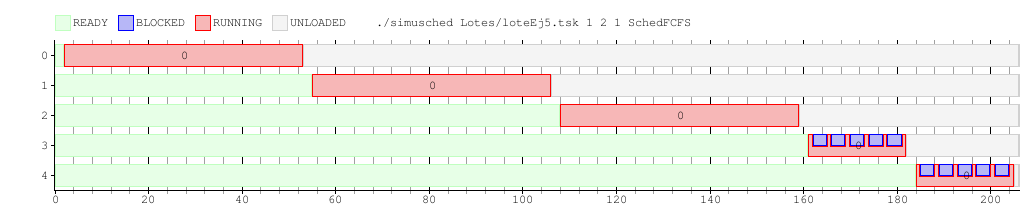
\includegraphics[width=1.1\textwidth]{imagenes/Ej6.png}
  \caption{loteEj5.tsk con FCFS}
\end{figure}

Del gráfico obtuvimos la siguiente tabla de tiempos para cada tarea\\

\begin{tabular}{ l | c | c | c | c | c | c | }
  \hline			
  pid & ciclos & inicio & fin & latencia & waiting time & tiempo total  \\
  \hline
0 & 51 & 0 & 53 & 2 & 2 & 53\\
1 & 51 & 0 & 106 & 55 & 55 & 106\\
2 & 51 & 0 & 159 & 108 & 108 & 159\\
3 & 21 & 0 & 182 & 161 & 161 & 182\\
4 & 21 & 0 & 205 & 184 & 184 & 205\\
\hline
\end{tabular}\\

Vemos que el gráfico y tiempos se parecen bastante a lo realizado para el SchedRR con quantum de 50 debido a que cuant más grande es el quantum, más tiempo permanece corriendo las tareas.